% Lab Writeup for Diode-Laser Spectroscopy Lab
% Adam Reyes, George Wong
% Advanced Lab FAll 2013

%edited by adam to include methods on interferometer theory and
%discussion of broadened line spacings


\documentclass[paper=a4, fontsize=11pt]{scrartcl} % A4 paper and 11pt font size
\usepackage[left=2.5cm,top=2.5cm,right=2.5cm,bottom=2.5cm]{geometry} 
\usepackage{amsmath}
\usepackage{graphicx}
\usepackage{sectsty}
\usepackage{fancyhdr}
\pagestyle{fancyplain}
\usepackage{subcaption}
\usepackage{wrapfig}
\usepackage[english]{babel}

\numberwithin{equation}{section}
\numberwithin{figure}{section} 
\numberwithin{table}{section}
%\setlength\parindent{0pt}

\fancyhead[R]{\thepage} 
\fancyhead[L]{Reyes, Wong} 
\fancyhead[C]{Saturated Absorption Spectroscopy} 
\fancyfoot[L]{} 
\fancyfoot[C]{} 
\fancyfoot[R]{} 

\newcommand{\horrule}[1]{\rule{\linewidth}{#1}}

\title{	
Saturated Absorption Spectroscopy of Rubidium
\horrule{0.5pt}
\normalfont \normalsize 
\textsc{Advanced Experimental Physics }
}

\author{Adam Reyes \\ George Wong} % Your name

\date{\normalsize\today} % Today's date or a custom date


\begin{document}
\maketitle
%%%%%%%%%Abstract%%%%%%%%%%
\noindent\textbf{Abstract:}
A diode-laser swept through the absorption bands of Rubidium was used
to measure the absorption spectrum of the Rubidium lines. With the use
of a pump beam, the saturated absorption of Rubidium was found and
used to investigate the fine structure of Rubidium. 


\section{Background}


\indent It is well understood that an electron bound to a nucleus in
some atom is restricted to a set of allowed energies, of which it can
be found in. These energies correspond to ``wavefunctions'', which are
eigenfunctions of the atom's energy Hamiltonian operator, that
describe the probability of finding that electron at a given point in
space. Because an electron is restricted to these allowed energies, it
can absorb energy only of an amount that is exactly the difference to
some other allowed energy, $\Delta E$, these are shown qualitatively
in Figure ~\ref{fig:energies}. 

 \begin{figure}[h] \begin{center}
  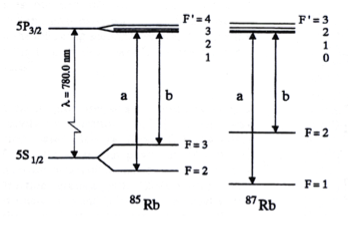
\includegraphics[height=60mm]{energy.png}
  \caption{\textbf{Energy Spectrum for Rubidium}\cite{caltech}. Lines
    represent allowed energies for a Rubidium atom. }
  \label{fig:energies}
\end{center} \end{figure}

A photon of light carries some energy that corresponds to its
frequency, given by: $E_\gamma = h\nu$, where $h$ is Planck's
constant. If a photon carries energy $E_\gamma = \Delta E$, the energy
of an allowed transition for an atomic electron, then the electron can
absorb the photon and transition to an excited state. Since there is
not a continuous spectrum of allowed energies the electron can only
absorb photons for specific frequencies. We now consider some source
of light, of varying frequency, is incident on a sample of some atom
and the intensity of the light is measured on the other side of the
sample. Since the atoms can only absorb particular frequencies of
light, and transmit all others, in a plot of the measured transmitted
intensity against light frequency, we would see dips in the
transmitted intensities at the frequencies that correspond precisely
to the allowed energy transitions of the atomic electrons, as in
Figure ~\ref{fig:broadening}. 

\begin{figure}[h] \begin{center}
  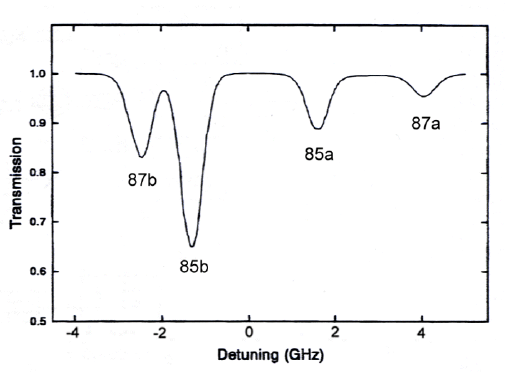
\includegraphics[height=60mm]{broadening.png}
  \caption{\textbf{Standard example of spectrum with Doppler broadening}\cite{caltech}}
  \label{fig:broadening}
\end{center} \end{figure}


\section{Doppler Broadened Absorption}
\label{sec:broad}

\subsection{Introduction}

An interesting feature of Figure ~\ref{fig:broadening} is that the
absorption peaks all have some width, with absorption bleeding into
frequencies around those corresponding to allowed transitions. This
phenomena is known as Doppler Broadening, and is a result of atoms in
the gas phase obeying a Maxwell Speed Distribution. For a light beam incident
on a sample of some gas, the velocity of the atoms in the sample will
have some component along the propagation direction of the light. For
atoms with velocity components along the direction of the light will,
in their rest frame, see the light being red-shifted towards a lower
frequency. Likewise in the rest frame of those atoms moving against
the incident direction of the light will see the light being
blue-shifted towards a higher frequency. Because of this the sample as
a whole can absorb light of frequencies off resonance from the
frequencies associated with the allowed transitions, leading to the
broadened peaks of Figures ~\ref{fig:broadening} and
~\ref{fig:absorb1}. 

\begin{figure}[h] \begin{center}
  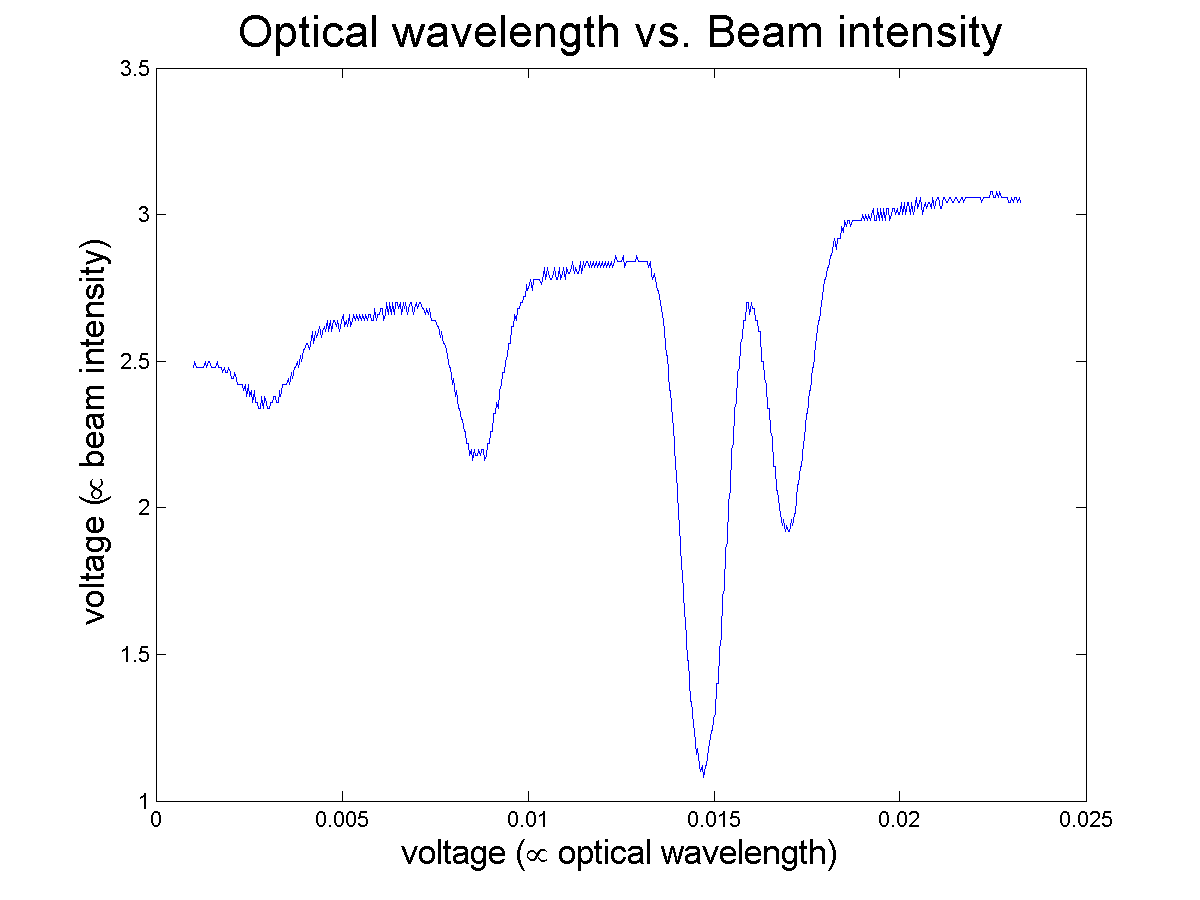
\includegraphics[height=80mm]{absorb3.png}
  \caption{\textbf{Intensity of Laser Beam with Varied Frequency through Rubidium Chamber} showing the effective absorption spectrum of Rubidium as a function of frequency (represented here as change in frequency over time). }
  \label{fig:absorb1}
\end{center} \end{figure}

\subsection{Methods}
\label{sec:dop:meth}
To observe a Doppler Broadened absorption spectrum we used a diode
laser aimed at a chamber of Rubidium gas held at $50^\circ$C. The
following steps were performed to absorb an absorption spectrum of Rubidium:

\begin{enumerate}
\item The provided laser was turned on and the current to the laser
  was increased until the beams was observed to be ``lasing''. This
  was the threshold of laser current associated with the beam, as viewed through
  the CCTV camera on a piece of paper, jumping discontinuously in intensity. 
\item The laser was aimed at and through the Rb gas chamber.
\item A ramp voltage was applied to the piezoelectric within the laser
  assembly. This voltage controlled the angle of incidence of the
  laser on a diffraction grating, effectively controlling the
  frequency of light incident on the gas chamber. 
\item A CCTV camera, capable of viewing infrared light was aimed as the Rb gas chamber. The incident current to the laser assembly was increased until florescence was seen.
\item A photoelectric diode, capable of reporting incoming light
  intensity in the form of voltage, was placed in the path of the beam
  exiting the Rubidium chamber.
\item The voltage from the diode was measured on an oscilloscope
  against ramp voltage to the piezo ($\propto$ frequency of light).
\item The voltage offset, frequency, and slope of the ramp were adjusted, as was the current to the laser. This was done until the absorption spectrum of both the $^{85}$Rb and $^{87}$Rb isotopes could be seen on the scope.
\item Several samples of the spectrum were taken. They are reproduced in Figures~\ref{fig:absorb1}$-$\ref{fig:absorb2}.
\item The voltage from the diode was then subtracted from the voltage of the ramp, with the scales of the two appropriately adjusted for compatibility. This allowed for observation of the spectrum without the ramp voltage artifact.
\end{enumerate}

\subsection{Results}
\begin{figure}[h] \begin{center}
  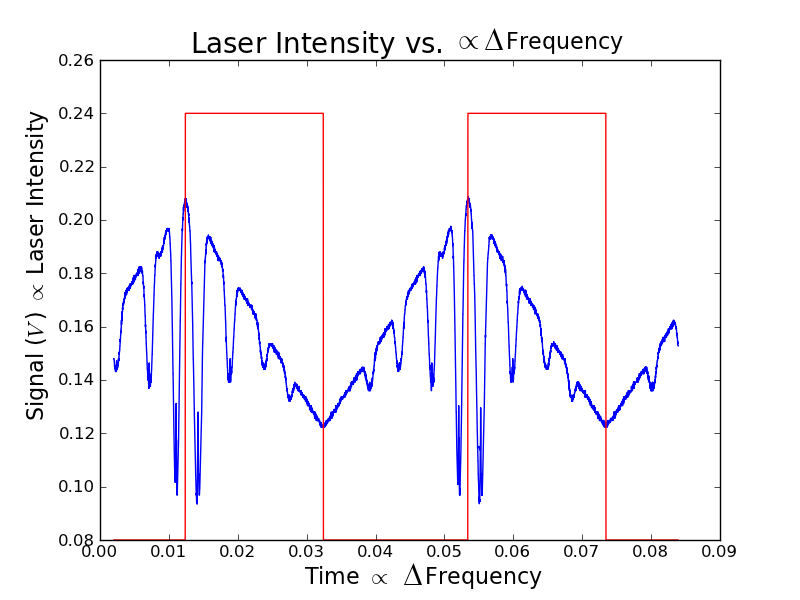
\includegraphics[height=80mm]{2-2-002.png}
  \caption{\textbf{Intensity of Laser Beam vs. Varying Laser Frequency
      with Pump}  shown over the course of approximately two full
    cycles in frequency. The red lines show the beginning and end of
    one ramp cycle.}
  \label{fig:absorb2}
\end{center} \end{figure}

\section{Michelson Interferometer}

\subsection{Introduction}

In order to interpret an absorption spectrum it is essential that we
know what frequency, or relative frequency, of light is incident on
our sample. Since our diffraction grating sweeps through its position
at a constant rate a simple Michelson Interferometer can be set up to
convert between the time of in our oscilloscope traces and a relative
frequency scale. The motivation being so we can measure the relative
frequencies of the different excited and ground states in our Rubidium
spectrums.

A Michelson Interferometer is made by splitting some beam of light
into two arms with a path length distance, $\Delta L$, between
them. The light is then recombined and sent into a detector. Because
of the difference in path length, when recombined the two beams will
be out of phase, and the combined beam's intensity will go as:
\begin{equation}
I \propto 1 + \cos \frac{4\pi \Delta Lf}{c}
\end{equation}
where $f$ is the frequency of light and $c$ is the speed of light. If
the frequency of the light is shifted, then the intensity will go as a
sinusoid, with period 
\begin{equation}
\label{eqn:T}
T = \frac{2\Delta L \delta f}{c}
\end{equation}
here $\delta f$ is corresponding change in frequency. Equation
~\ref{eqn:T} can be inverted to give $\delta f$:
\begin{equation}
\label{eqn:df}
\delta f = \frac{c}{2\Delta L T}
\end{equation}

\subsection{Methods}

The laser from Section ~\ref{sec:broad} was used with the same
settings tuned to the absorption lines of Rubidium. A diagram of the
interferometer can be found in Figure~\ref{fig:setup} as the part of
the apparatus beginning with the reflected beam from the first beam splitter. The following was
done to set up the apparatus:
\begin{enumerate}
\item The beam incident to the wedge was split into two (using a beam splitter) and the stronger beam was sent to the interferometer setup (described in the following steps). The weaker beam was sent to the probe-pump beam setup as given above.
\item The interferometer beam was sent to a 50-50 beam splitter placed so as to create a new perpendicular beam.
\item In the path of the original beam was placed a mirror which reflected light back at the beam splitter.
\item In the path of the new beam (leaving the splitter at $90^\circ$
  to the original beam) was placed another mirror. This mirror
  reflected the beam back to the splitter. This mirror was placed as
  far away from the splitter as possible, so as to maximize the
  difference in distance both beams (original and split) traveled. We
  measured a $\Delta L$ of $1.7971 \pm 0.0001$m, by counting the
  number of holes on the optics table. 
\item The two beams (off of both mirrors) were aligned after passing through the beam splitter one last time.
\item This aligned beam was directed into a photoelectric diode to measure light intensity.
%\item Measurements of absorption spectra (with pump beam to point out hyperfine splitting) were made alongside interferometer intensity. Figure~\ref{fig:int_1} represents these data.
\end{enumerate}

\subsection{Results}
\begin{figure}[h] \begin{center}
  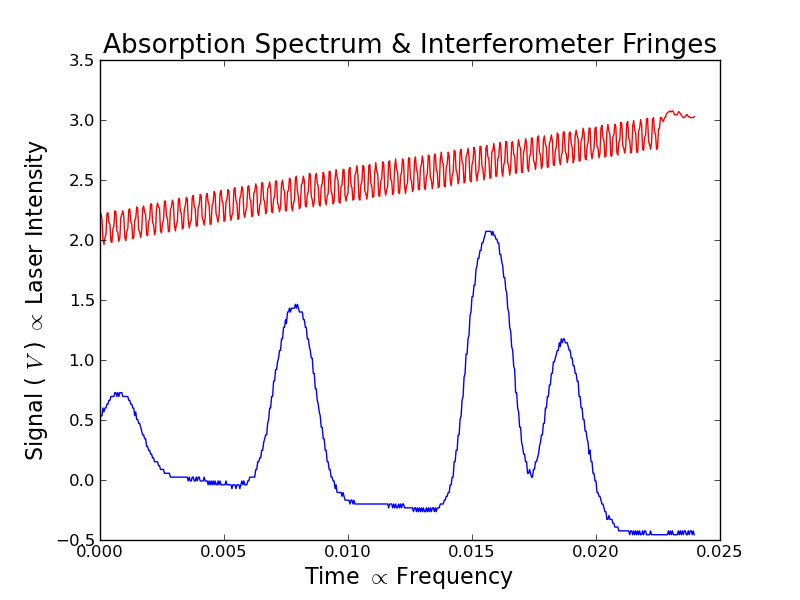
\includegraphics[height=70mm]{4-1-009.png}
  \caption{\textbf{Laser Intensity \& Interferometer Beam Intensity over Change in Frequency} demonstrating the changing intensity (fringes) generated by the interferometer over the same interval as the intensity incident from the laser beam traveling through the Rubidium chamber. }
  \label{fig:int_1}
\end{center} \end{figure}

Figure ~\ref{fig:int_1} shows our interference patter (shown in red)
alongside a Rubidium absorption spectrum. To establish a conversion
between time and frequency, the number of periods in a given interval of
the interference pattern were counted. Using Equation ~\ref{eqn:df}
the $\frac{\delta f}{T}$ can be calculated to give a conversion
between time and frequency. We established a $\frac{\delta f}{T}$ of
$0.004 \pm
.002\frac{\normalfont{GHz}}{\normalfont{ms}}$. Figure~\ref{fig:detuning}
shows the absorption spectrum of Rubidium against the detuning from
the largest peak. 

The error here is dominated by that from the determination of $\Delta L$ and
could be reduced by having a larger difference in the length of the
two arms of the interferometer. Because of the fixed length of the BNC
cable coming from the photo-diode detector we were limited to roughly
half of the length of the optics bench for the long arm.  

\begin{figure}[h] \begin{center}
  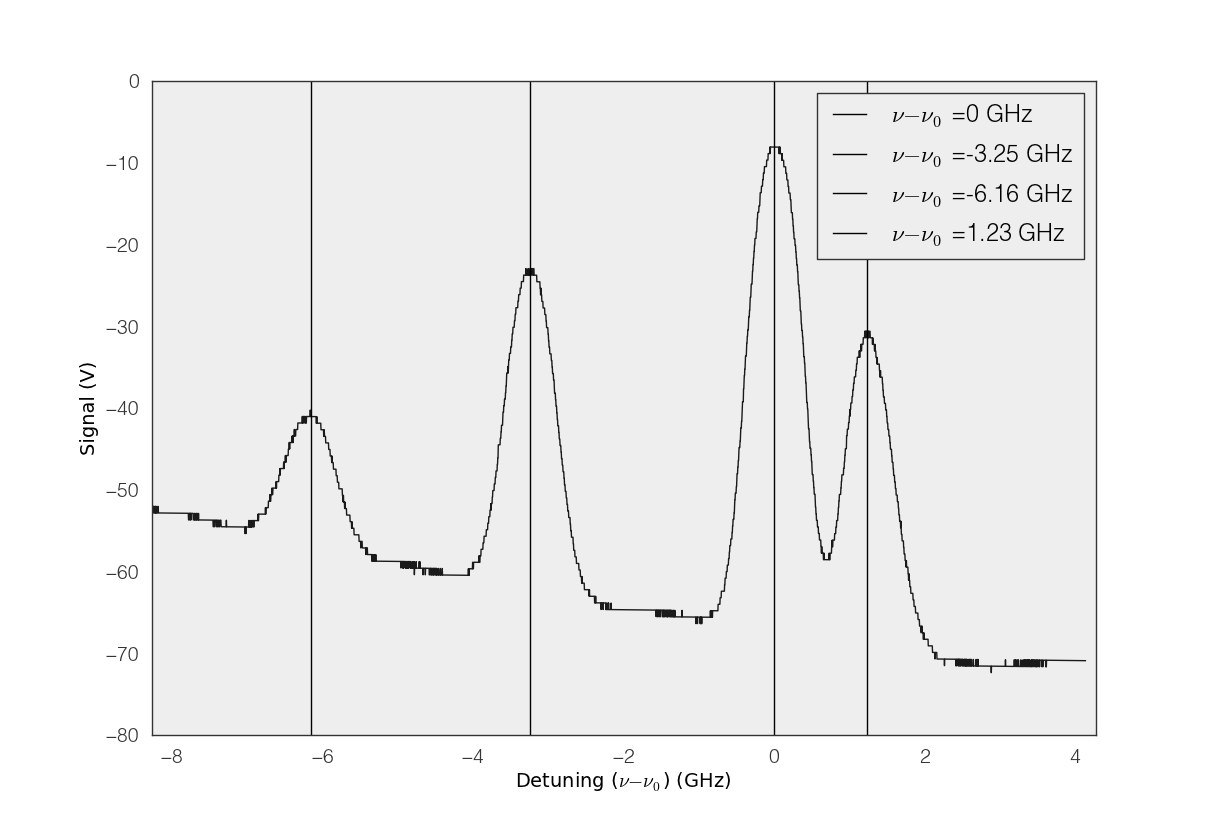
\includegraphics[height=80mm]{Detuning.png}
  \caption{\textbf{Absorption Spectrum of Rubidium } with
      interferometrically determined detuning centered around the largest peak. }
  \label{fig:detuning}
\end{center} \end{figure}

\section{Saturated Absorption}

\subsection{Introduction}
\label{sec:satabintro}
We can see in Figure ~\ref{fig:energies} that the 5P$_{\frac{3}{2}}$
ground state of both Rubidium isotopes is split into two levels give by the F' quantum
number. This splitting is due to coupling of the electron's spin to
its ``orbit'' and is called the hyperfine structure. 

However, we notice in the absorption spectrums so far discussed
(Figures ~\ref{fig:absorb1}, ~\ref{fig:broadening}), that we see only
the wide doppler broadened lines expected for the un-split
5P$_{\frac{3}{2}}$ state. This is because, as we can see in Figure
~\ref{fig:energies}, that the 5P$_{\frac{3}{2}}$ splittings are much
more closely spaced than the ground state lines and more importantly
closer together than the doppler broadening for each
transition. Because the doppler broadening is wider than the
separation of the excited state splittings they can not be seen in a
regular absorption experiment.

To get around this we now consider two collinear beams incident on the
Rubidium sample in opposite directions. One beam, called the pump
beam, is to have intensity much greater than the other. The weaker
beam is called the probe beam, and is the one whose intensity is to be
measured after exiting the Rubidium gas. For atoms in the gas with velocity
component along the beam direction the light will be shifted in
opposite frequency directions for the respective beams since the two beams are
going in opposing directions. This will, as before, result in the
typical doppler broadening off-resonance with respect to the
transitions. For atoms with zero velocity component along the light
propagation direction there is no frequency shift for either beam, and
both beams can be absorbed by the atom. Because the pump beam is so
intense it will saturate these atoms, stationary in the beam
direction, in the excited state, preventing the probe beam from being
absorbed and increasing its transmission percentage when the incident
light is on resonance, allowing for the fine structure of Rubidium to
be seen in an absorption spectrum using this set up.

Another consequence of the close frequency proximity of the split
5P$_{\frac{3}{2}}$ states is the phenomena of cross-over
peaks. Consider two closely spaced resonant lines at frequencies
$\nu_1$ and $\nu_2$ and a light frequency of $\nu_{\gamma} = \frac{\nu_1 +
  \nu_2}{2}$. Because of doppler broadening there will be a ``false''
peak at $\nu_{\gamma}$. 
\subsection{Methods}
\label{sec:satabmeth}
\begin{figure}[h] \begin{center}
  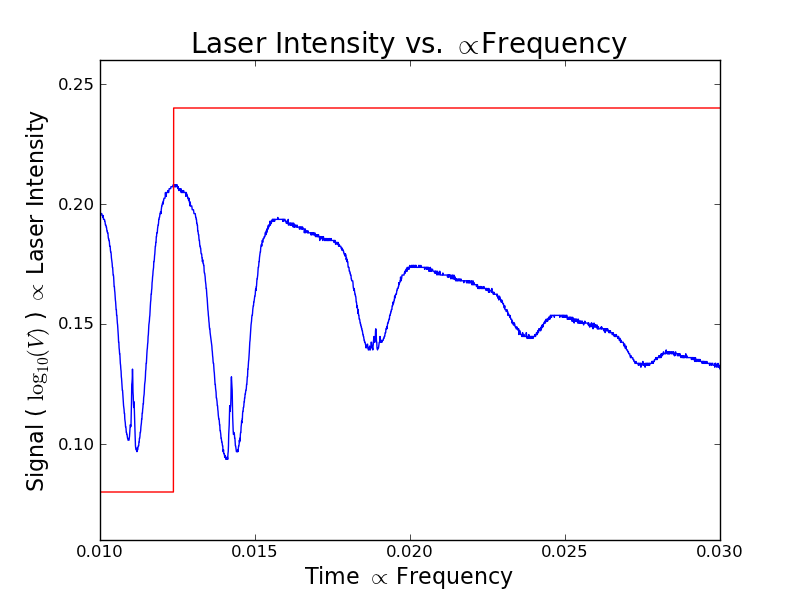
\includegraphics[height=80mm]{2-2-002-zoom.png}
  \caption{\textbf{Intensity of Laser Beam vs. Varying Laser Frequency with Pump} shown over a restricted interval. A Pump beam has clearly been added, as hyperfine splitting is more easily observable. }
  \label{fig:withPump_1}
\end{center} \end{figure}
The same Rubidium cell and laser from Sec.~\ref{sec:dop:meth} were
used in this experiment. A diagram of our apparatus is shown in Figure
~\ref{fig:setup}. The following steps were carried out in performing
this experiment. 
\begin{enumerate}
\item The beam, instead of being reflected by a mirror into the
  chamber, is sent into a 2$^\circ$ wedge and the reflected beams sent
  into the Rubidium chamber and into two photo-diode detectors on the
  other side. The transmitted beam is reflected around
  the chamber.
\item The beam directed around the chamber was aimed at a 50-50 beam
  splitter that reflects the beam into the chamber to be the pump beam.
\item The pump beam was then aligned to be collinear with one of the
  beams coming from the wedge (probe beam). The probe beam signal is
  shown in Figures~\ref{fig:satabsorb1} and~\ref{fig:withPump_1}
\item The signal from the probe beam was subtracted electronically
  from the reference signal coming from other wedged beam, shown in Figure~\ref{fig:scaled_1}. 
\end{enumerate}

\clearpage
\begin{figure}[h] \begin{center}
  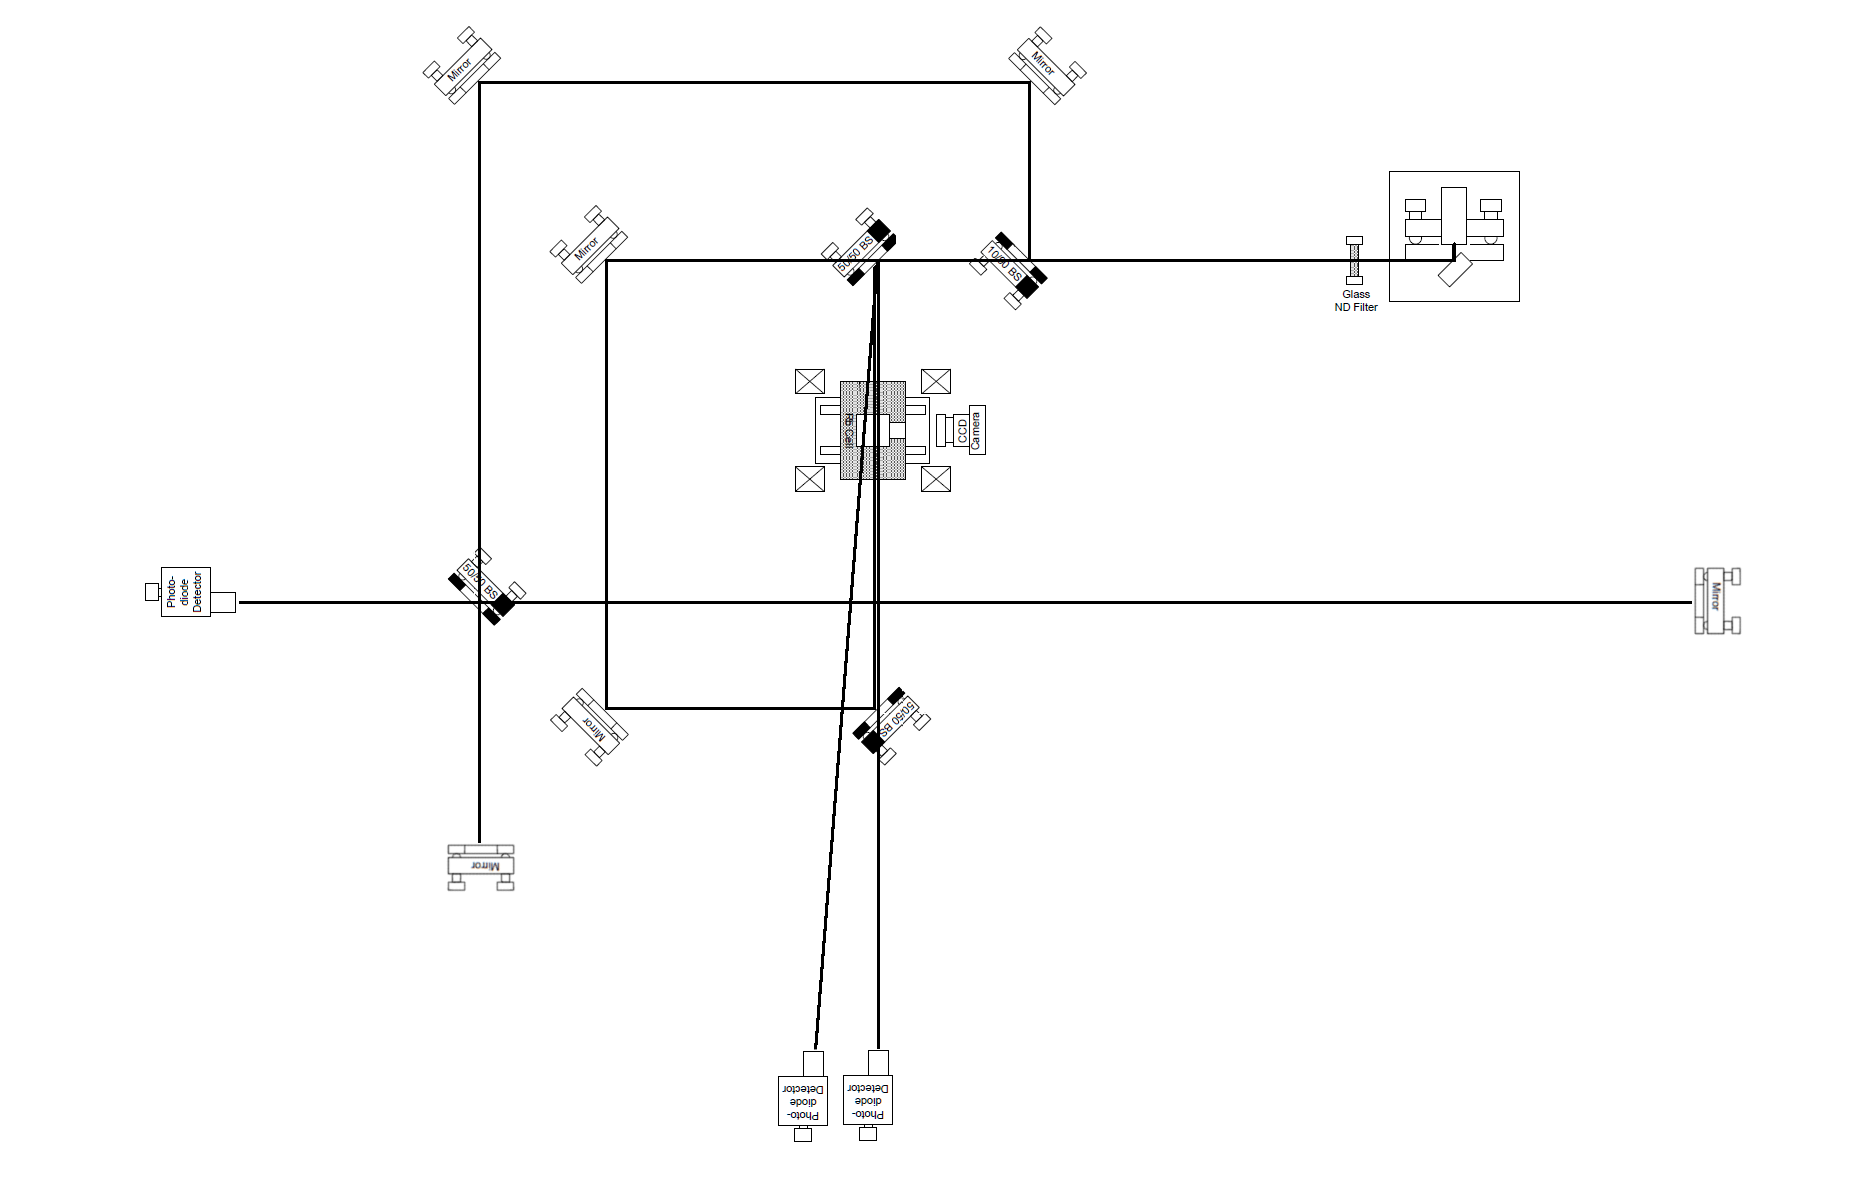
\includegraphics[height=6in, angle = 90]{full.png}
  \caption{\textbf{Overall final set up of apparatus} showing
    placement of all beam splitters, mirrors, and various other
    devices to simultaneously measure the saturated absorption
    spectrum and take interferometric measurements. }
  \label{fig:setup}
\end{center} \end{figure}
\clearpage

\begin{figure}[h] \begin{center}
  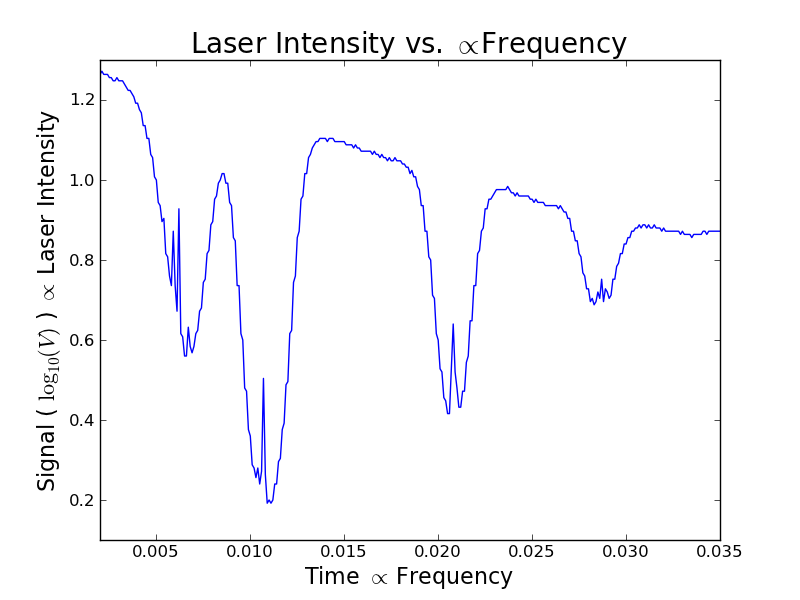
\includegraphics[height=100mm]{3-1-001.png}
  \caption{\textbf{Hyperfine splitting} as observed with the experimental set up used for this examination (sample shows intensity from combination of pump and probe beams). }
  \label{fig:satabsorb1}
\end{center} \end{figure}

\begin{figure}[h] \begin{center}
  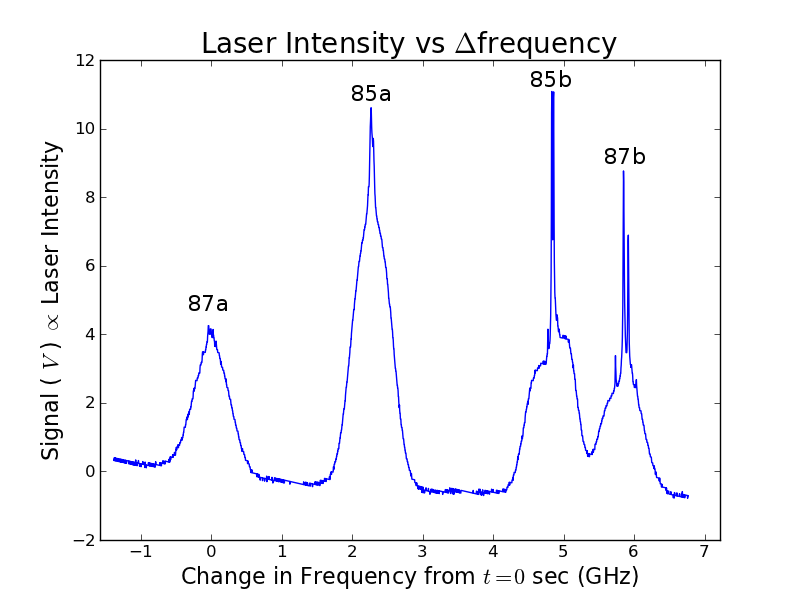
\includegraphics[height=70mm]{4-2-009.png}
  \caption{Saturated absorption \textbf{Plot of intensity vs. frequency shift} for data sample 1. }
  \label{fig:scaled_1}
\end{center} \end{figure}

\subsection{Results}

%%%%%%%%HERE GOES TABLES AND STUFF FROM OTHER DRAFT%%%%%%%%%%%%%%%%%%%%%%%

\begin{figure}[h] \begin{center}
  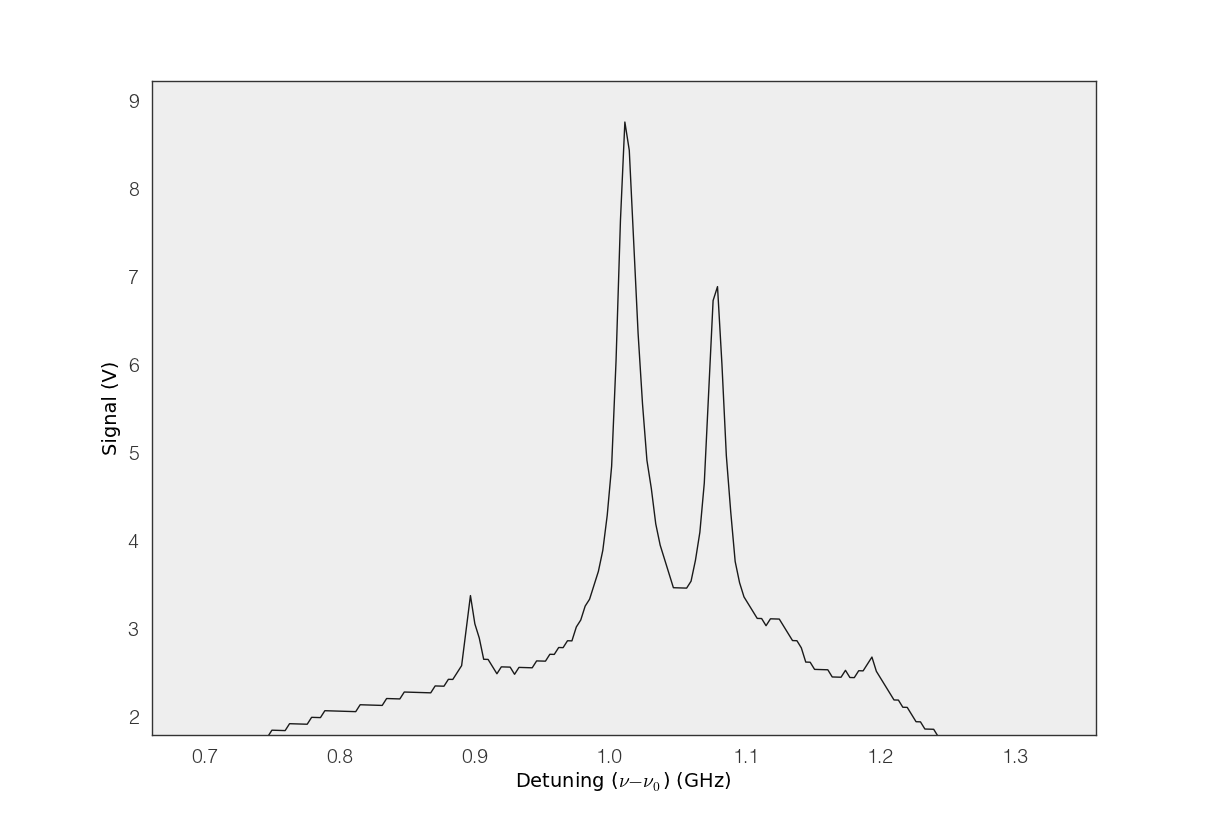
\includegraphics[height=70mm]{detune1.png}
  \caption{Saturated absorption \textbf{Plot of intensity
      vs. detuning} from $^{85}$Rb b line in
    Figure~\ref{fig:scaled_1}, zoomed in to show fine structure. 87b
    line shown here.}
  \label{fig:det1}
\end{center} \end{figure}

\begin{figure}[h] \begin{center}
  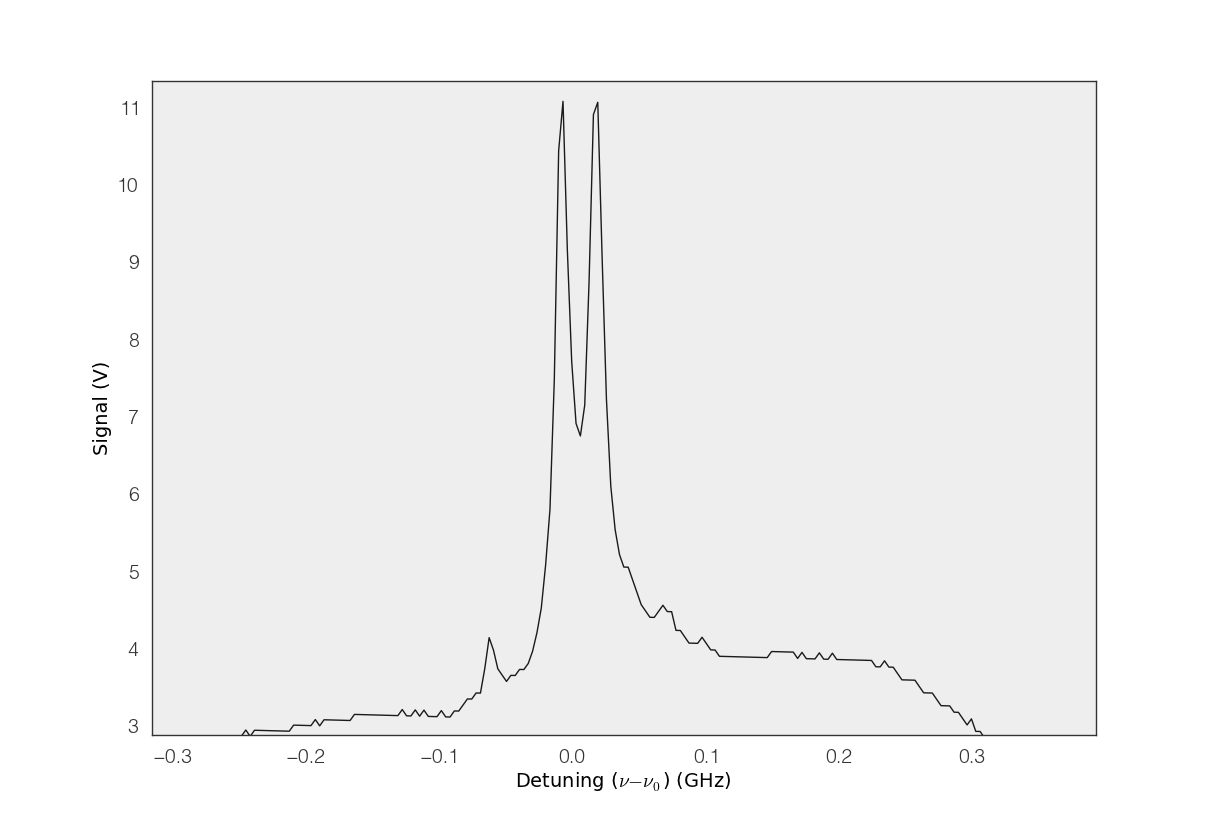
\includegraphics[height=70mm]{detune2.png}
  \caption{Saturated absorption \textbf{Plot of intensity vs. detuning} from $^{85}$Rb b line in
    Figure~\ref{fig:scaled_1}, zoomed in to show fine structure. 85b
    line shown here.}
  \label{fig:det2}
\end{center} \end{figure}

We would expect to see evidence of the crossover peaks in
Figures~\ref{fig:det1} and ~\ref{fig:det2}, which shows a blown up
view of the 87 and 85 b lines, so labeled in Figure
~\ref{fig:scaled_1}. What we can see, in both cases, is two well
defined peaks of large amplitude. In figure ~\ref{fig:det1} we can see
two small peaks in the absorption at around 0.9 and 1.2 GHz detuning
and possibly another at 1.1 GHz. As shown in
Figure~\ref{fig:energies}, both $^{85}$ and $^{87}$ Rubidium have
their excited state split into four energy levels. Here we count
four and possibly a fifth. Five peaks would be conclusive evidence of
one of these being a cross-over peak. We would expect that a
cross-over peak would be of greater intensity than the regular
resonance peaks, because they have contribution from multiple excited
state transitions instead of just one. Because there are two peaks
with significantly greater amplitude, we are inclined to believe that
these are cross-over peaks, but this would leave two resonance peaks
that are not here shown.

In the 85b spectrum (Figure~\ref{fig:det2}) we see again two peaks
with large amplitude and two smaller peaks at around $\pm$ 0.8 GHz
detuning. If we again take the two larger peaks to be due to
cross-overs then there are two more resonance peaks not found. 

As can be seen in our doppler-subtracted spectrum
(Figure~\ref{fig:scaled_1}),  the resulting spectrum is not ideal. We
had great difficulty in finding the right combination of the two
signals to exactly subtract the doppler broadening, and so if the
missing peaks were of small enough amplitude it is reasonable that
they might have been lost in the process. 



\begin{thebibliography}{99}
\bibitem{vanier}Jacques Vanier. Relaxation in rubidium-87 and the
  rubidium maser. Phys. Rev., 168:129-149, 1968.
\bibitem{harvard}"Rubidium Fluoresence." Cfa.harvard.edu. Harvard,
  n.d. Web.
\bibitem{caltech}Caltech Department of Physics. Saturated Absorption
Spectroscopy. Caltech
\end{thebibliography}


%%%%%%%%%%%FIGURES%%%%%%%%%%%%

\section{Figures}

\subsection{please remove this for final draft}

\input{figures.tex}

\end{document}
